% Provenance (never printed): see sources/outline_sources.md (Year 3:
% energy-balance models, the one-layer model recalled; ice-albedo feedback
% and multiple equilibria; how general circulation models are built and
% evaluated).
% Brief: sources/book5/BRIEFS.md, ch. 22. Curves from
% figdata/bachelor-3/budyko_sellers.py (the zero-dimensional model and
% Budyko's latitudinal model; the brief's ebm_0d is folded into it) and
% two_layer.py. Exercise and problem values in the Book 5 scratch calculator
% calc/ch22.py. The model planet, model X and the ensemble of exercise 12 are
% invented.
\chapter{Climate Models}\label{ch:b3:climate-models}

Take the sunlight that reaches the Earth, \qty{340}{W/m^2} averaged over
the globe, and a law for the infrared it sends back to space fitted to
thirty years of a reanalysis of the observations. Let the planet's albedo rise from that
of open ground and sea to that of ice as the surface cools. Balance the two
fluxes, and the equation has three solutions: a planet at
\qty{14}{\celsius}, close to the mean of the real one; a planet at
\qty{8}{\celsius}; and a planet at \qty{-46}{\celsius}, frozen from pole to
pole. Climate models, from these few lines to programs run on the largest
computers, are tools for asking which climate a given planet has, how it
gets there, and how it changes when its energy balance is disturbed.
% ledger: nasa:solar-mean, data:b5-ncep-air, data:b3-ncep, budyko69:albedo

\begin{recall}
The black body, the Stefan--Boltzmann law, the greenhouse effect and the
one-layer model of the atmosphere are in the physics books; the albedo and
the Earth's energy budget in the school books. The outgoing longwave
radiation, the emission temperature and the meridional heat transport are
in the Year~1 volume, in its chapter on radiation and heat transport. The
ice--albedo feedback and the snowball Earth are in the Year~2 volume, in
its chapter on the Precambrian Earth; the effective radiative forcing, the
climate feedback parameter $\lambda < 0$, the equilibrium climate
sensitivity (ECS) and the transient climate response (TCR) in its chapter
on anthropogenic climate change; numerical weather prediction and the
ensemble forecast in its chapter on weather systems. The equations of
motion on the rotating Earth, with the \omterm{def:b3:gfd-foundations:hydrostatic}{hydrostatic approximation}, are in
Chapter~\ref{ch:b3:gfd-foundations}.
\end{recall}

\section{The energy balance of a planet}\label{sec:b3:climate-models:zero-d}

Averaged over the sphere and over a year, each square metre at the top of
the atmosphere receives $Q = S_0/4 = \qty{340}{W/m^2}$, a quarter of the
solar irradiance $S_0 = \qty{1360}{W/m^2}$. A fraction $\alpha$, the
planetary albedo, is reflected; the rest, $Q(1 - \alpha)$, is absorbed and
must be sent back to space as infrared. A black body would emit $\sigma
T^4$; the Earth's outgoing longwave radiation (OLR) is smaller, because of
the greenhouse effect, and over the range of surface temperatures found on
the Earth it is close to a straight line,
\[
\text{OLR} = A + BT ,
\]
with $T$ the surface temperature in degrees Celsius. In 1969 Budyko fitted
such a law to the outgoing radiation computed for 260 stations, with a correction for
cloudiness $n$: $I = a + bT - (a_1 + b_1T)n$, $a = 14.0$, $b = 0.14$, $a_1 =
3.0$ and $b_1 = 0.10$ in \unit{kcal.cm^{-2}} per month, with a scatter under
\qty{5}{\percent}. For a mean cloudiness of 0.5 it gives $A =
\qty{199}{W/m^2}$ and $B = \qty{1.43}{W.m^{-2}.\celsius^{-1}}$. The annual
\omterm{def:b3:atmospheric-dynamics:eddy}{zonal means} of the NCEP--NCAR Reanalysis~1 for 1991--2020, weighted by area,
give $A = \qty{211.9}{W/m^2}$ and $B = \qty{1.816}{W.m^{-2}.\celsius^{-1}}$,
with a scatter of \qty{10}{W/m^2} about the line. These values are used
below.
% ledger: nasa:solar-mean, budyko69:olr, data:b5-ncep-air, data:b3-ncep

\begin{definition}[Energy-balance model]\label{def:b3:climate-models:ebm}
An \emph{energy-balance model}\index{energy-balance model} is a climate
model that computes a surface temperature --- a single global mean, or a
mean over each latitude --- from the balance of the sunlight absorbed, the
infrared emitted to space and, if the temperature depends on latitude, the
heat carried towards the poles. In its zero-dimensional form,
\[
C\,\frac{\mathrm dT}{\mathrm dt} = Q\big(1 - \alpha(T)\big) - (A + BT) ,
\]
where $C$ is the heat capacity per unit area of the part of the system that
warms with the surface.
\end{definition}

With $\alpha = 0.30$ the equilibrium is $T = (238 - 211.9)/1.816 =
\qty{14.4}{\celsius}$; the area mean of the reanalysis is
\qty{14.2}{\celsius}. A forcing $F$, such as that of a change of carbon
dioxide, adds to the right-hand side. Near an equilibrium the response is
governed by the climate feedback parameter $\lambda$ of the Year~2 volume:
with the albedo fixed, $\lambda = -B$.
% ledger: earth:albedo, data:b5-ncep-air

\begin{theorem}[Response time of a one-box climate]\label{thm:b3:climate-models:response}
Let a climate be in equilibrium, and let a constant forcing $F$ be switched
on at $t = 0$. If the departure $T'$ from the equilibrium obeys $C\,\mathrm
dT'/\mathrm dt = F + \lambda T'$ with $C > 0$ and $\lambda < 0$ constant,
then
\[
T'(t) = -\frac{F}{\lambda}\Big(1 - \mathrm e^{-t/\tau}\Big), \qquad
\tau = -\frac{C}{\lambda} .
\]
The new equilibrium is $-F/\lambda$, and the climate covers the fraction $1
- \mathrm e^{-1} = \num{0.63}$ of the way in the time $\tau$.
\end{theorem}

\begin{proof}
$T'_\infty = -F/\lambda$ makes the right-hand side vanish. The difference
$u = T' - T'_\infty$ obeys $C\,\mathrm du/\mathrm dt = \lambda u$, so $u =
u(0)\,\mathrm e^{\lambda t/C}$, with $u(0) = F/\lambda$.
\end{proof}

The heat capacity that matters over a few years is that of the upper ocean.
The two-layer emulator of the sixth assessment report of the
Intergovernmental Panel on Climate Change, calibrated on 44 climate models,
gives the surface layer $C = \qty{8.1}{W.yr.m^{-2}.\celsius^{-1}}$, the heat
capacity of a layer of sea water \qty{62}{m} deep. With $\lambda = -B$ the
response time is $8.1/1.816 = \num{4.5}\text{ years}$. The real climate also warms
the deep ocean, much more slowly; Section~\ref{sec:b3:climate-models:two-layer}
adds it.
% ledger: ar6sm7:two-layer, teos10:cp0, data:b5-ncep-air

\section{Ice, albedo and multiple equilibria}\label{sec:b3:climate-models:multiple}

The ice--albedo feedback of the Year~2 volume makes the albedo depend on
temperature. Take $\alpha = 0.62$ for a planet whose surface is below
$T_I = \qty{-10}{\celsius}$, the albedo of ice in Budyko's model, $\alpha
= 0.30$ above $T_F = \qty{+10}{\celsius}$, and a straight line between, as
the ice retreats. The ramp is a choice of this chapter; any albedo that
rises as the planet cools gives the same picture.
% ledger: budyko69:albedo, earth:albedo

\begin{definition}[Multiple climate equilibria; saddle-node bifurcation]\label{def:b3:climate-models:multiple-equilibria}
A climate model has \emph{multiple climate equilibria}\index{multiple climate equilibria}
when, for the same external conditions, it has more
than one steady state. An equilibrium is stable if a small departure from
it decays, unstable if it grows. A \emph{saddle-node
bifurcation}\index{saddle-node bifurcation} is the value of a parameter at
which a stable and an unstable equilibrium meet and disappear together.
\end{definition}

\begin{proposition}[Three equilibria and their stability]\label{prop:b3:climate-models:three}
Write $N(T) = Q(1 - \alpha(T)) - (A + BT)$ for the net downward flux. An
equilibrium $T^*$, $N(T^*) = 0$, is stable if $N'(T^*) < 0$ and unstable if
$N'(T^*) > 0$. With the ramp above, $N' = -B$ on the snowball and
ice-free branches, which are stable wherever they exist, and $N' = -B -
Q\,\mathrm d\alpha/\mathrm dT$ on the ramp, which is unstable when $Q\,
|\mathrm d\alpha/\mathrm dT| > B$. For $Q = \qty{340}{W/m^2}$ the model has
three equilibria, \qty{-45.5}{\celsius} (stable), \qty{7.8}{\celsius}
(unstable) and \qty{14.4}{\celsius} (stable).
\end{proposition}

\begin{proof}
Near $T^*$, $C\,\mathrm dT'/\mathrm dt = N'(T^*)T'$, which decays if
$N'(T^*) < 0$ and grows if $N'(T^*) > 0$. On the ramp $\mathrm d\alpha/
\mathrm dT = -0.32/20 = \qty{-0.016}{\celsius^{-1}}$, so $N' = -1.816 + 340
\times 0.016 = \qty{+3.62}{W.m^{-2}.\celsius^{-1}}$. The snowball branch,
$T = (340\times0.38 - 211.9)/1.816 = \qty{-45.5}{\celsius}$, lies below
$T_I$; the warm one, \qty{14.4}{\celsius}, above $T_F$; on the ramp,
$340(0.54 + 0.016\,T) = 211.9 + 1.816\,T$ gives $T = \qty{7.8}{\celsius}$.
\end{proof}

\begin{omfigure}
\begin{tikzpicture}
\begin{groupplot}[group style={group size=2 by 1, horizontal sep=1.5cm},
  width=0.48\linewidth, height=0.4\linewidth,
  tick label style={font=\scriptsize}, label style={font=\small}, title style={font=\small}]
\nextgroupplot[xlabel={$T$ (\unit{\celsius})}, ylabel={flux (\unit{W/m^2})},
  xmin=-60, xmax=40, ymin=80, ymax=270, title={balance at $Q = \qty{340}{W/m^2}$},
  legend style={font=\scriptsize, at={(0.03,0.97)}, anchor=north west}]
% computed in figdata/bachelor-3/budyko_sellers.py
\addplot[omThm, thick] table[x=T, y=asr] {figdata/out/bachelor-3-budyko_sellers-asr.dat};
\addlegendentry{absorbed sunlight}
\addplot[omDef, thick] table[x=T, y=olr] {figdata/out/bachelor-3-budyko_sellers-olr.dat};
\addlegendentry{$A + BT$}
\addplot[only marks, mark=*, mark size=2pt, forget plot] coordinates {(-45.55,129.2) (14.38,238.0)};
\addplot[only marks, mark=o, mark size=2pt, thick, forget plot] coordinates {(7.81,226.07)};
\node[font=\scriptsize, anchor=north west] at (axis cs:-45.55,125) {snowball};
\draw[black!60] (axis cs:7.81,226.07) -- (axis cs:16,200);
\node[font=\scriptsize, anchor=north west, inner sep=1pt] at (axis cs:16,200) {unstable};
\nextgroupplot[xlabel={$S_0$ (\unit{W/m^2})}, ylabel={$T$ (\unit{\celsius})},
  xmin=1000, xmax=2200, ymin=-70, ymax=100, title={equilibria and hysteresis},
  scaled x ticks=false, xticklabel style={/pgf/number format/1000 sep={}}]
\addplot[black!40, densely dotted, forget plot] coordinates {(1360,-70) (1360,100)};
\addplot[omMeth, thick] table[x=S, y=T] {figdata/out/bachelor-3-budyko_sellers-eqwarm.dat};
\addplot[omThm, thick] table[x=S, y=T] {figdata/out/bachelor-3-budyko_sellers-eqcold.dat};
\addplot[black!60, thick, dashed] table[x=S, y=T] {figdata/out/bachelor-3-budyko_sellers-eqmid.dat};
\draw[->, thick, black!70] (axis cs:1314.6,8) -- (axis cs:1314.6,-45);
\draw[->, thick, black!70] (axis cs:2039.4,-8) -- (axis cs:2039.4,77);
\node[font=\scriptsize, anchor=south, black!60, fill=white, inner sep=1pt] at (axis cs:1360,84) {today};
\node[font=\scriptsize, omMeth, anchor=north west] at (axis cs:1700,32) {warm};
\node[font=\scriptsize, omThm, anchor=north] at (axis cs:1620,-40) {snowball};
\end{groupplot}
\end{tikzpicture}

\par\smallskip{\small The zero-dimensional \omterm{def:b3:climate-models:ebm}{energy-balance model} with an
ice--albedo ramp and the OLR law fitted to the NCEP--NCAR Reanalysis~1.
Left, the absorbed sunlight and the emitted infrared for today's sunlight:
they cross three times; filled circles are stable, the open one unstable.
Right, the equilibrium temperature against the solar constant, stable
branches solid, the unstable one dashed. Lowering the Sun from today's
value cools the warm planet until the warm branch ends at
\qty{1315}{W/m^2}, and the climate falls to the snowball; it stays frozen
until the Sun is raised to \qty{2039}{W/m^2}, where it jumps back to a
very hot planet, far beyond the range in which the straight-line OLR
holds.}\label{fig:b3:climate-models:zero-d}
\end{omfigure}
% ledger: nasa:solar-mean, data:b5-ncep-air, budyko69:albedo, earth:albedo

As $Q$ falls, the warm equilibrium cools and the ramp equilibrium warms.
They meet at the top of the ramp, $T = T_F$, where $Q(1 - 0.30) = A +
10B$: $Q = \qty{328.7}{W/m^2}$, a solar constant of \qty{1315}{W/m^2},
\qty{3.3}{\percent} below today's. That is a \omterm{def:b3:climate-models:multiple-equilibria}{saddle-node bifurcation}: below
it the only equilibrium is the snowball, and the climate falls into it.
Raising the Sun again does not bring the warm planet back: the snowball
branch ends only where its temperature reaches $T_I$, $Q(1 - 0.62) = A -
10B$, at a solar constant of \qty{2039}{W/m^2}, \qty{50}{\percent} above
today's. Between the two, the state of the planet depends on its history:
the model has hysteresis. In the real Neoproterozoic the way out of the
snowball of the Year~2 volume was not a brighter Sun but the carbon dioxide
of volcanoes, building up over millions of years until the greenhouse
forcing reached the deglaciation threshold; the ice line then retreated to
the poles in a few thousand years.
% ledger: hoffman17:hysteresis

\section{The Budyko--Sellers model}\label{sec:b3:climate-models:budyko-sellers}

A single temperature has no ice line. In 1969 Budyko let the temperature
depend on latitude and asked how far a reduction of the sunlight would push
the ice towards the equator.

\begin{definition}[Budyko--Sellers model]\label{def:b3:climate-models:budyko-sellers}
A \emph{Budyko--Sellers model}\index{Budyko--Sellers model} is an
\omterm{def:b3:climate-models:ebm}{energy-balance model} in which the annual mean temperature $T(x)$ depends on
$x = \sin\varphi$, $\varphi$ the latitude, the hemispheres being symmetric.
At each latitude
\[
C\,\frac{\partial T}{\partial t} = Qs(x)\big(1 - \alpha(x)\big) - (A + BT) - D(x) ,
\]
where $s(x)$ is the annual insolation of the latitude divided by its global
mean, $D(x)$ the divergence of the poleward heat transport, and the albedo
takes its ice value poleward of the ice line $x_s$, where $T$ falls below a
critical temperature $T_c$. Budyko wrote $D = \beta(T - \bar T)$, a
relaxation towards the global mean $\bar T$; in the diffusive form, $D =
-\mathcal D\,\partial_x\big[(1 - x^2)\,\partial_xT\big]$.
\end{definition}

The factor $x = \sin\varphi$ is chosen because equal intervals of $x$ hold
equal areas of the sphere, so that a global mean is $\int_0^1\cdot\,\mathrm
dx$. Budyko found $\beta = \qty{0.235}{kcal.cm^{-2}}$ per month and per
degree, \qty{3.74}{W.m^{-2}.\celsius^{-1}}, from the observed distribution
of temperature with latitude. He set the albedo to 0.62 on the ice and to 0.50 at its edge,
where the ice is broken, and took the present ice edge at a mean latitude
of \ang{72} N; the critical temperature is the one that puts the edge
there.
% ledger: budyko69:transport, budyko69:albedo

\begin{proposition}[The ice line of Budyko's model]\label{prop:b3:climate-models:iceline}
Let $F(x_s) = \int_0^{x_s}s\,\mathrm dx$ be the fraction of the sunlight that
falls equatorward of the ice line, and $\bar\alpha = \alpha_FF + \alpha_I(1 -
F)$ the mean albedo weighted by sunlight. In a steady state of Budyko's
model,
\[
B\bar T = Q(1 - \bar\alpha) - A, \qquad
T(x) = \frac{Qs(x)\big(1 - \alpha(x)\big) - A + \beta\bar T}{B + \beta} ,
\]
and an ice line at $x_s$, where $T = T_c$ with the edge albedo $\alpha_e$,
needs
\[
Q(x_s) = \frac{(B + \beta)T_c + A(1 + \beta/B)}{s(x_s)(1 - \alpha_e) +
(\beta/B)\big(1 - \bar\alpha(x_s)\big)} .
\]
An ice line is stable where $\mathrm dQ/\mathrm dx_s > 0$ and unstable
where $\mathrm dQ/\mathrm dx_s < 0$.
\end{proposition}

\begin{proof}
Integrate the steady balance over $0 \le x \le 1$: the transport term
vanishes, because $\int_0^1(T - \bar T)\,\mathrm dx = 0$, and $\int_0^1
s(1 - \alpha)\,\mathrm dx = 1 - \bar\alpha$; this gives $\bar T$. The
steady balance at each $x$ is then linear in $T(x)$. Setting $T(x_s) = T_c$
and replacing $\bar T$ by its value gives the last formula, linear in $Q$.
The stability condition is admitted: it follows from linearising the
time-dependent model about the steady state.
\end{proof}

Its meaning is the one of the zero-dimensional model: along a stable branch
a little more sunshine pushes the ice line poleward. The temperature at
which the edge sits today fixes $T_c = \qty{-12.3}{\celsius}$; the
reanalysis gives \qty{-15.8}{\celsius} at \ang{72}, the mean of the two
hemispheres. The model's profile below is cooler than the observed one in the
tropics and much warmer near the poles: a single coefficient $\beta$ cannot
fit the whole profile. Its global mean,
\qty{12.8}{\celsius}, and its equator, \qty{22.8}{\celsius}, are close to
the observed \qty{14.2}{\celsius} and \qty{25.7}{\celsius}.
% ledger: data:b5-ncep-air, data:b3-ncep, budyko69:albedo

\begin{omfigure}
\begin{tikzpicture}
\begin{groupplot}[group style={group size=2 by 1, horizontal sep=1.5cm},
  width=0.48\linewidth, height=0.42\linewidth,
  tick label style={font=\scriptsize}, label style={font=\small}, title style={font=\small}]
\nextgroupplot[xlabel={$Q/Q_0$}, ylabel={ice-line latitude (\unit{\degree})},
  xmin=0.95, xmax=1.25, ymin=-3, ymax=93, ytick={0,15,30,45,60,75,90},
  title={ice line against sunlight}, clip=false,
  scaled x ticks=false, xticklabel style={/pgf/number format/fixed, /pgf/number format/precision=2}]
% computed in figdata/bachelor-3/budyko_sellers.py
\addplot[black!40, densely dotted] coordinates {(1,-3) (1,93)};
\addplot[omMeth, thick] table[x=q, y=lat] {figdata/out/bachelor-3-budyko_sellers-icestable.dat};
\addplot[black!60, thick, dashed] table[x=q, y=lat] {figdata/out/bachelor-3-budyko_sellers-iceunstable.dat};
\addplot[omThm, thick] coordinates {(0.95,0) (1.2249,0)};
\addplot[omMeth, thick] coordinates {(1.0069,90) (1.25,90)};
\addplot[only marks, mark=*, mark size=2pt] coordinates {(1,72) (1,0) (0.9713,47.65)};
\addplot[only marks, mark=o, mark size=2pt, thick] coordinates {(1,30.15)};
\node[font=\scriptsize, anchor=west] at (axis cs:1.005,72) {today};
\draw[black!60] (axis cs:0.9713,47.65) -- (axis cs:1.02,50);
\node[font=\scriptsize, anchor=west, align=left] at (axis cs:1.02,50) {glaciation threshold};
\node[font=\scriptsize, omThm, anchor=south] at (axis cs:1.06,1) {snowball};
\node[font=\scriptsize, omMeth, anchor=north] at (axis cs:1.15,89) {no ice};
\nextgroupplot[xlabel={latitude (\unit{\degree})}, ylabel={$T$ (\unit{\celsius})},
  xmin=0, xmax=90, xtick={0,15,30,45,60,75,90}, ymin=-35, ymax=32, title={temperature today},
  legend style={font=\scriptsize, at={(0.03,0.03)}, anchor=south west}]
\addplot[omDef, thick] table[x=lat, y=tmodel] {figdata/out/bachelor-3-budyko_sellers-profile.dat};
\addlegendentry{Budyko model}
\addplot[black, thick, mark=*, mark size=0.9pt] table[x=lat, y=tobs] {figdata/out/bachelor-3-budyko_sellers-obs.dat};
\addlegendentry{reanalysis}
\addplot[black!50, densely dashed] coordinates {(0,-12.26) (90,-12.26)};
\addlegendentry{$T_c$}
\end{groupplot}
\end{tikzpicture}

\par\smallskip{\small Budyko's latitudinal model with the OLR law of the
reanalysis and the insolation of each latitude. Left, the sunlight $Q/Q_0$
needed to hold the ice line at each latitude: stable branch solid, unstable
dashed. Today, $Q/Q_0 = 1$, three states coexist: the ice line at \ang{72}
(stable), at \ang{30} (unstable) and the snowball. The stable branch ends
at its minimum, \ang{47.7} and \num{0.9713}: with less sunlight there, the
ice runs to the equator. Right, the model's temperature today against the
annual \omterm{def:b3:atmospheric-dynamics:eddy}{zonal mean} of the NCEP--NCAR Reanalysis~1, 1991--2020, averaged over
the two hemispheres; the ice line is where the model's curve, with the
albedo of the edge, reaches $T_c$.}\label{fig:b3:climate-models:budyko}
\end{omfigure}
% ledger: data:b5-ncep-air, data:b3-ncep, budyko69:albedo, budyko69:transport

The stable branch has a minimum. With these values it lies at \ang{47.7},
for $Q/Q_0 = \num{0.9713}$: a fall of \qty{2.87}{\percent} in the sunlight
brings the ice to the middle latitudes, and any further fall sends it to
the equator. Budyko found a smaller threshold with his own coefficients: a
fall of \qty{1.6}{\percent} brought his ice to a mean latitude of about
\ang{50}, after which it advanced to the equator of itself and the mean
temperature fell to several tens of degrees below zero. The fit of the OLR
and the albedos move the number; the shape of the curve, its minimum and the
runaway beyond it do not. The diffusive form of the model, solved with
Legendre polynomials in $x$, gives the same shape (exercise~\ref{exo:b3:climate-models:10}
treats a planet without ice).
% ledger: budyko69:threshold, hoffman17:hysteresis

\section{Two-layer models}\label{sec:b3:climate-models:two-layer}

The response time of the one-box model, a few years, is that of the upper
ocean. Below it the deep ocean takes up heat for centuries, and while it
does the surface stays cooler than its equilibrium.

\begin{definition}[Two-layer energy-balance model]\label{def:b3:climate-models:two-layer}
A \emph{two-layer energy-balance model}\index{two-layer energy-balance model}
represents the climate by a surface layer of temperature anomaly $T$
and heat capacity $C$, and a deep ocean of temperature anomaly $T_d$ and
heat capacity $C_d$, coupled by a heat exchange coefficient $\gamma > 0$:
\[
C\,\frac{\mathrm dT}{\mathrm dt} = F + \lambda T - \gamma(T - T_d), \qquad
C_d\,\frac{\mathrm dT_d}{\mathrm dt} = \gamma(T - T_d) .
\]
\end{definition}

\begin{theorem}[Fast and slow responses]\label{thm:b3:climate-models:two-layer}
Let $\lambda < 0$, $\gamma > 0$, $C, C_d > 0$, and let a constant forcing
$F$ start at $t = 0$ from equilibrium. Then
\[
T(t) = -\frac{F}{\lambda}\Big(1 - a_f\,\mathrm e^{-t/\tau_f} - a_s\,\mathrm
e^{-t/\tau_s}\Big), \qquad a_f + a_s = 1 ,
\]
where $1/\tau_f$ and $1/\tau_s$ are the roots of $r^2 - \big((\gamma -
\lambda)/C + \gamma/C_d\big)r - \lambda\gamma/(CC_d) = 0$. When $C \ll C_d$,
\[
\tau_f \approx \frac{C}{\gamma - \lambda}, \qquad
\tau_s \approx \frac{C_d(\gamma - \lambda)}{-\lambda\gamma}, \qquad
a_f \approx \frac{-\lambda}{\gamma - \lambda} .
\]
\end{theorem}

\begin{proof}
The equilibrium is $T = T_d = -F/\lambda$. The departures from it obey
$\mathrm d\vec u/\mathrm dt = M\vec u$ with
\[
M = \begin{pmatrix} (\lambda - \gamma)/C & \gamma/C\\ \gamma/C_d &
-\gamma/C_d\end{pmatrix}, \qquad
\operatorname{tr}M = -\frac{\gamma - \lambda}{C} - \frac{\gamma}{C_d},
\qquad \det M = \frac{-\lambda\gamma}{CC_d} > 0 ,
\]
so both eigenvalues $-r$ are real and negative, $r$ satisfying the quadratic
of the statement. Each component of $\vec u$ is a combination of $\mathrm
e^{-t/\tau_f}$ and $\mathrm e^{-t/\tau_s}$; $T(0) = 0$ gives $a_f + a_s =
1$. If $C \ll C_d$ the larger root is close to the trace, $(\gamma -
\lambda)/C$, and the smaller is the determinant divided by it. On the fast
time scale the deep ocean has not moved, $T_d \approx 0$, and the surface
settles at $F/(\gamma - \lambda)$, the fraction $-\lambda/(\gamma - \lambda)$
of the final warming: that is $a_f$.
\end{proof}

The emulator of the assessment, calibrated to 44 models, has $C =
\qty{8.1}{W.yr.m^{-2}.\celsius^{-1}}$, $C_d = \qty{110}{W.yr.m^{-2}.\celsius^{-1}}$
and $\gamma = \qty{0.62}{W.m^{-2}.\celsius^{-1}}$; its feedback parameter is
sampled about $\lambda = \qty{-1.33}{W.m^{-2}.\celsius^{-1}}$. These values
give $\tau_f = \num{4.1}\text{ years}$ and $\tau_s = \num{262}\text{ years}$, with $a_f =
0.67$: \qty{62}{\percent} of the warming comes within a decade, most of the
rest over centuries. The emulator also multiplies the heat exchange in the first
equation by an efficacy $\varepsilon = 1.34$, which slows the surface
further; it is set to 1 here.
% ledger: ar6sm7:two-layer

\begin{omfigure}
\begin{tikzpicture}
\begin{groupplot}[group style={group size=2 by 1, horizontal sep=1.4cm},
  width=0.48\linewidth, height=0.4\linewidth,
  tick label style={font=\scriptsize}, label style={font=\small}, title style={font=\small},
  ylabel={warming (\unit{\celsius})}]
\nextgroupplot[xlabel={years after the step}, xmin=0, xmax=500, ymin=0, ymax=6.6,
  title={abrupt quadrupling},
  legend style={font=\scriptsize, at={(0.97,0.03)}, anchor=south east}]
% computed in figdata/bachelor-3/two_layer.py
\addplot[omDef, thick] table[x=t, y=T] {figdata/out/bachelor-3-two_layer-abrupt.dat};
\addlegendentry{surface $T$}
\addplot[omThm, thick] table[x=t, y=Td] {figdata/out/bachelor-3-two_layer-abrupt.dat};
\addlegendentry{deep ocean $T_d$}
\addplot[black!60, densely dashed] coordinates {(0,5.91) (500,5.91)};
\addlegendentry{equilibrium}
\nextgroupplot[xlabel={years from the start}, xmin=0, xmax=140, ymin=0, ymax=6.2,
  xtick={0,35,70,105,140}, title={\qty{1}{\percent} per year},
  legend style={font=\scriptsize, at={(0.03,0.97)}, anchor=north west}]
\addplot[omDef, thick] table[x=t, y=T] {figdata/out/bachelor-3-two_layer-ramp.dat};
\addlegendentry{surface $T$}
\addplot[omThm, thick] table[x=t, y=Td] {figdata/out/bachelor-3-two_layer-ramp.dat};
\addlegendentry{deep ocean $T_d$}
\addplot[black!60, densely dashed] table[x=t, y expr=\thisrow{F}/1.33] {figdata/out/bachelor-3-two_layer-ramp.dat};
\addlegendentry{$-F/\lambda$}
\addplot[black!40, densely dotted, forget plot] coordinates {(70,0) (70,6.2)};
\addplot[only marks, mark=*, mark size=1.8pt, forget plot] coordinates {(70,1.987) (70,2.955)};
\node[font=\scriptsize, anchor=west] at (axis cs:72,1.75) {TCR};
\node[font=\scriptsize, anchor=east] at (axis cs:68,3.2) {ECS};
\end{groupplot}
\end{tikzpicture}

\par\smallskip{\small The two-layer model with the mean parameters of the
emulator of the sixth assessment and the forcing $F_{2\times} =
\qty{3.93}{W/m^2}$ of a doubling. Left, an abrupt quadrupling of carbon
dioxide: \qty{62}{\percent} of the final \qty{5.9}{\celsius} after 10
years, \qty{78}{\percent} after 100 and \qty{95}{\percent} after 500.
Right, carbon dioxide rising by \qty{1}{\percent} a year: at the doubling,
year 70, the surface has warmed by \qty{1.99}{\celsius}, the TCR of the
model, while the equilibrium warming for that forcing, its ECS, is
\qty{2.95}{\celsius}; the surface lags because the deep ocean is still
taking up heat.}\label{fig:b3:climate-models:two-layer}
\end{omfigure}
% ledger: ar6sm7:two-layer, ipcc:erf-2xco2, ar6ch7:tcr

The model gives the two sensitivities of the Year~2 volume. Its ECS is
$-F_{2\times}/\lambda = 3.93/1.33 = \qty{2.95}{\celsius}$. During a ramp
lasting decades the deep ocean, with its time scale of centuries, has hardly
warmed, and the surface is close to the fast balance $T \approx F/(\gamma -
\lambda)$: the TCR is about $3.93/1.95 = \qty{2.0}{\celsius}$, against
\qty{1.99}{\celsius} for the integration. With the efficacy, $\gamma$ is
replaced by $\kappa = \varepsilon\gamma = \qty{0.84}{W.m^{-2}.\celsius^{-1}}$,
and $\text{TCR} = F_{2\times}/(\kappa - \lambda) = \qty{1.8}{\celsius}$,
the best estimate assessed by the report, which also assesses an ECS of
\qty{3}{\celsius}, \emph{likely} 2.5 to \qty{4}{\celsius} (\emph{high
confidence}). The assessment finds that the differences of $\gamma$ and
$\varepsilon$ between models explain 10 to \qty{20}{\percent} of their
spread of TCR.
% ledger: ar6sm7:two-layer, ar6ch7:emulator, ar6ch7:tcr, ipcc:ecs, ipcc:erf-2xco2

A model this simple, tuned to reproduce the global temperature of a large
model, is an emulator. The assessment ran a simple climate model whose temperature module is
this two-layer model as an ensemble of a million members, sampled over the
ranges of its parameters, and kept the 2237 members that reproduced the
observed warming since 1850, the heat taken up by the ocean, the carbon
dioxide of the air and the fraction of emissions that stays in it.
% ledger: ar6sm7:two-layer, ar6ch1:esm

\section{General circulation models}\label{sec:b3:climate-models:gcm}

An \omterm{def:b3:climate-models:ebm}{energy-balance model} is given its feedbacks and its transport; a
\omterm{def:b3:climate-models:gcm}{general circulation model} computes them from the laws of physics.

\begin{definition}[General circulation model; dynamical core; parameterisation]\label{def:b3:climate-models:gcm}
A \emph{general circulation model}\index{general circulation model} (GCM)
is a numerical model of the atmosphere, of the ocean, or of both coupled,
that solves the equations of motion, continuity and energy of a fluid on
the rotating Earth --- for the atmosphere, with the \omterm{def:b3:gfd-foundations:hydrostatic}{hydrostatic
approximation}, the ``primitive equations'' --- on a three-dimensional
grid covering the globe, stepping forward in time. Its \emph{dynamical
core}\index{dynamical core} is the part that solves these equations for
the motions the grid resolves. A
\emph{parameterisation}\index{parameterisation} represents the effect on
the resolved variables of a process smaller than a grid cell --- clouds,
convection, turbulence, gravity waves --- by a formula in the resolved
variables, with parameters that the modellers choose.
\end{definition}

The resolution decides what must be parameterised. The \omterm{def:b3:climate-models:gcm}{general circulation
models} of 1990 had grid cells about \qty{500}{km} across; the global models
of the last assessment, about \qty{100}{km}; regional models, 25 to
\qty{50}{km}, and a dedicated intercomparison has explored global grids of
about 50, 25 and even \qty{10}{km}. A single convective cloud is much smaller than a global cell: convection
is parameterised, and regional models fine enough to resolve it are now
included in the intercomparisons.
% ledger: ar6ch1:faq-resolution, ar6ch1:models, ar6ch1:parameterization

\begin{omfigure}
\centering
\begin{tikzpicture}[>=stealth, font=\small, x=1cm, y=1cm]
% grid of columns
\fill[omThm!8] (3.2,0) rectangle (4.8,4.2);
\foreach \i in {0,...,5} \draw[black!40] (\i*1.6,0) -- (\i*1.6,4.2);
\foreach \j in {0,...,6} \draw[black!40] (0,\j*0.7) -- (8,\j*0.7);
\fill[omMeth!25] (0,-0.25) rectangle (3.2,0);
\fill[black!25] (3.2,-0.25) rectangle (8,0);
\node[font=\scriptsize, anchor=north] at (1.6,-0.3) {ocean};
\node[font=\scriptsize, anchor=north] at (5.6,-0.3) {land};
% resolved flow
\foreach \y in {0.35,2.45,3.85} {\draw[->, omMeth, thick] (1.0,\y) -- (2.2,\y); \draw[->, omMeth, thick] (5.8,\y) -- (7.0,\y);}
% parameterised processes in the highlighted column
\draw[->, omDef, very thick] (4.0,0.55) -- (4.0,2.6);
\draw[->, omThm, thick, decorate, decoration={snake, amplitude=0.6mm, segment length=2mm, post length=1mm}] (3.45,4.6) -- (3.45,0.15);
\draw[->, omDef!70!black, thick, decorate, decoration={snake, amplitude=0.6mm, segment length=2mm, post length=1mm}] (4.55,0.15) -- (4.55,4.6);
\fill[white] (3.75,2.95) circle (0.22); \fill[white] (4.05,3.05) circle (0.27); \fill[white] (4.35,2.95) circle (0.2);
\draw[black!60, thick] (3.75,2.95) circle (0.22); \draw[black!60, thick] (4.05,3.05) circle (0.27); \draw[black!60, thick] (4.35,2.95) circle (0.2);
\draw[black!70, thick] (3.62,0.22) .. controls (3.55,0.62) and (4.1,0.62) .. (3.95,0.32) .. controls (3.85,0.15) and (3.7,0.35) .. (3.82,0.42);
% labels
\node[omMeth, font=\scriptsize, align=center, fill=white, inner sep=1pt] at (1.6,1.4) {resolved winds:\\the dynamical core};
\node[font=\scriptsize, align=left, anchor=west] (c) at (8.3,3.1) {clouds};
\node[font=\scriptsize, align=left, anchor=west] (v) at (8.3,1.8) {convection};
\node[font=\scriptsize, align=left, anchor=west] (r) at (8.3,4.4) {sunlight and infrared};
\node[font=\scriptsize, align=left, anchor=west] (t) at (8.3,0.4) {turbulence near the surface};
\draw[black!50] (c.west) -- (4.6,3.05);
\draw[black!50] (v.west) -- (4.05,1.8);
\draw[black!50] (r.west) -- (4.6,4.4);
\draw[black!50] (t.west) -- (3.95,0.4);
\node[font=\scriptsize, black!70, anchor=west, align=left] at (8.3,-0.4) {parameterised in the column};
\draw[decorate, decoration={brace, amplitude=4pt, mirror}] (3.2,-0.7) -- (4.8,-0.7)
  node[midway, below=4pt, font=\scriptsize] {one cell, about \qty{100}{km}};
\end{tikzpicture}

\par\smallskip{\small A slice through the grid of a global model, not to
scale. Between cells, the winds and the transports of heat and moisture are
computed by the \omterm{def:b3:climate-models:gcm}{dynamical core}; inside each column, the processes smaller
than the cell --- clouds, convection, the transfer of sunlight and
infrared, the turbulence of the lowest layer --- are parameterised, from
the resolved temperature, humidity and wind of the
column.}\label{fig:b3:climate-models:grid}
\end{omfigure}
% ledger: ar6ch1:faq-resolution, ar6ch1:parameterization

\begin{definition}[Earth system model]\label{def:b3:climate-models:esm}
An \emph{Earth system model}\index{Earth system model} (ESM) is a \omterm{def:b3:climate-models:gcm}{general
circulation model} of the atmosphere and the ocean coupled to models of the
sea ice, the land surface and its vegetation, and of the carbon cycle, so
that the concentrations of greenhouse gases and the properties of the
surface can respond to the climate they help to set.
\end{definition}

\omterm{def:b3:climate-models:esm}{Earth system models} are the most complex models used by the assessment. In
the 1990s the coupled atmosphere--ocean models were the state of the art;
by the 2010s land, vegetation and the carbon cycle had been added, and
ice-sheet models are being coupled to them. Most of their projections are
nevertheless run with prescribed concentrations of the greenhouse gases;
only the emission-driven runs let the model's carbon cycle compute them.
Between the \omterm{def:b3:climate-models:ebm}{energy-balance models} and the ESMs lies a hierarchy of models
of intermediate complexity, cheap enough to be run for many thousands of
years without a supercomputer.
% ledger: ar6ch1:models, ar6ch1:esm

\begin{omfigure}
\centering
\begin{tikzpicture}[>=stealth, font=\small,
  rung/.style={draw=omMeth!70, fill=omMeth!6, rounded corners=2pt, minimum height=0.85cm,
    text width=0.54\linewidth, align=left, inner sep=4pt},
  rname/.style={font=\small\bfseries, text width=0.2\linewidth, align=right, anchor=east}]
\node[rung] (e0) at (0,0) {one global temperature; sunlight in, $A + BT$ out};
\node[rung] (e1) at (0,1.15) {temperature by latitude, poleward transport, an ice line};
\node[rung] (e2) at (0,2.3) {surface layer and deep ocean; tuned to a large model, an emulator};
\node[rung] (e3) at (0,3.45) {atmosphere and ocean on a 3-D grid: dynamical core and parameterisations};
\node[rung] (e4) at (0,4.6) {a GCM with sea ice, land, vegetation and the carbon cycle};
\node[rname] at ([xshift=-6pt]e0.west) {zero-dimensional\\EBM};
\node[rname] at ([xshift=-6pt]e1.west) {Budyko--Sellers};
\node[rname] at ([xshift=-6pt]e2.west) {two-layer EBM};
\node[rname] at ([xshift=-6pt]e3.west) {GCM};
\node[rname] at ([xshift=-6pt]e4.west) {Earth system\\model};
\draw[->, thick, black!60] ([xshift=10pt]e0.south east) -- ([xshift=10pt]e4.north east)
  node[midway, right, font=\scriptsize, align=left] {more processes,\\more computing};
\end{tikzpicture}

\par\smallskip{\small The ladder of the models of this chapter. Each rung
adds processes that the one below had to be given; the lower rungs are
cheap enough to be run a million times, the upper ones need
supercomputers.}\label{fig:b3:climate-models:ladder}
\end{omfigure}
% ledger: ar6ch1:models, ar6ch1:esm, ar6sm7:two-layer

\begin{definition}[Spin-up]\label{def:b3:climate-models:spin-up}
The \emph{spin-up}\index{spin-up (of a model)} of a climate model is its
integration under constant forcing, from an initial state, until its slow
components --- above all the deep ocean and the carbon stores --- have
stopped drifting; the experiments start from the state it reaches.
\end{definition}

The two-layer model shows why a \omterm{def:b3:climate-models:spin-up}{spin-up} is long: its slow time scale is
\num{262}~years, and after three of them, nearly eight centuries, the
drift is still \qty{5}{\percent} of the initial imbalance. The assessment
notes that the different strategies used to spin up the models affected
their performance.
% ledger: ar6sm7:two-layer, ar6ch1:models

\begin{omfigure}
\centering
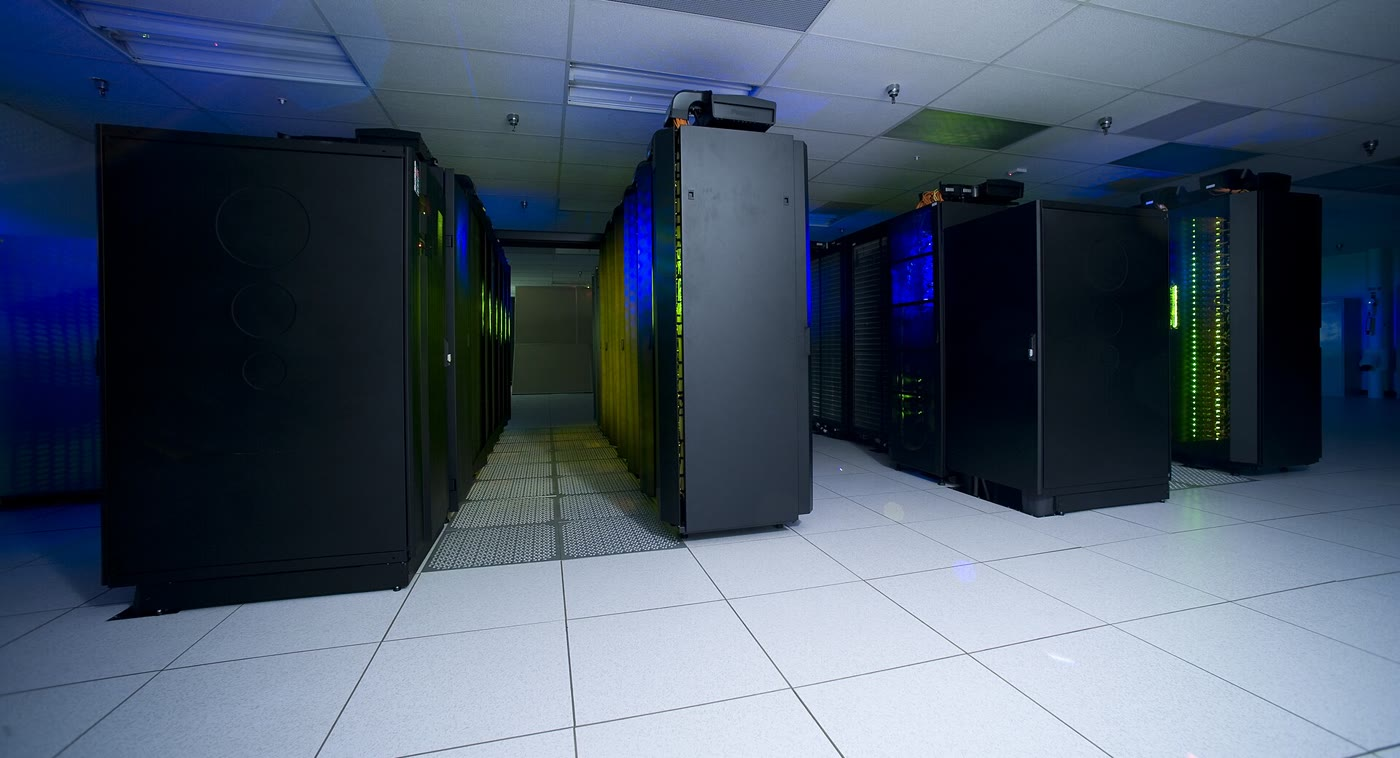
\includegraphics[width=0.7\linewidth]{images/book5/b3-nccs-supercomputer.jpg}

\par\smallskip{\small Racks of a supercomputer at the NASA Center for
Climate Simulation, Goddard Space Flight Center, in 2010 (NASA, public
domain). The equations of a global model are solved numerically on such
high-performance computers.}\label{fig:b3:climate-models:supercomputer}
\end{omfigure}
% ledger: photo:b3-nccs, ar6ch1:esm

\section{Evaluating models}\label{sec:b3:climate-models:evaluation}

A model is tested against the observed climate; the trouble is that it has
also been adjusted to it. Each \omterm{def:b3:climate-models:gcm}{parameterisation} has parameters whose
acceptable range is set by physics and observation, and as the components
are assembled the modellers refine them until the simulated climate meets a
set of tuning targets: the mean climate --- for example, a mean temperature
close to the observed one under today's sunlight --- regional features, or
the trends of the historical period. Only then is the model released for
the intercomparisons.
% ledger: ar6ch1:models, ar6ch1:parameterization, ar6ch1:large-ensembles

\begin{definition}[Model intercomparison project]\label{def:b3:climate-models:cmip}
A \emph{model intercomparison project}\index{model intercomparison project}
is a coordinated set of experiments --- the same forcings, the
same protocols, the same outputs --- run by many modelling groups with
their own models, so that the results can be compared. The Coupled Model
Intercomparison Project (CMIP) runs in successive phases; its sixth phase,
CMIP6, was a key line of evidence of the sixth assessment.
\end{definition}

\begin{dated}{2021}
Of 29 modelling groups of CMIP6 that reported how they tuned, 23 did not
tune their model to the warming observed during the historical period, and
25 did not tune its ECS: the sensitivity of most models is an emergent
property, not an input. On average the CMIP6 models have a higher ECS and
TCR than those of the previous phase, and a wider spread than the ranges
assessed by the report; in some models this was traced to the feedback of
the clouds of middle and high latitudes. Some of the most sensitive models
reproduce the observed recent warming and the climates of the past less
well. The assessment therefore did not take its ranges of ECS and TCR from
the models directly, but from the understanding of the feedback processes,
the instrumental record, the past climates and \omterm{def:b3:climate-models:evaluation}{emergent constraints}; it treats the most sensitive models as a guide to
outcomes of low likelihood and high impact (\emph{high confidence}).
\end{dated}
% ledger: ar6ch1:models, ar6ch7:cmip6-sensitivity

\begin{definition}[Large ensemble; emergent constraint]\label{def:b3:climate-models:evaluation}
A \emph{large ensemble}\index{large ensemble} is a set of many simulations
by a single model, with the same forcings over the same period, that differ
only in their initial states. An \emph{emergent
constraint}\index{emergent constraint} is a relationship, found across an
ensemble of different models, between an observable quantity of the
present climate and a quantity of the future one, such as the ECS; the
observed value of the first then narrows the range of the second.
\end{definition}

The climate is chaotic, so tiny differences of the initial state send the
members of a \omterm{def:b3:climate-models:evaluation}{large ensemble} along different paths: the spread of the
members measures the internal variability, and their mean the forced
response. \omterm{def:b3:climate-models:evaluation}{Large ensembles} of several models supported the assessment. An
\omterm{def:b3:climate-models:evaluation}{emergent constraint} needs a physical reason. Across a few dozen models,
thousands of observables can be tried, and some will correlate with the
ECS by chance; the assessment kept those with a physical basis, many of
them about the clouds of the tropics, and warned that a bias shared by all
the models of the ensemble defeats the method.
% ledger: ar6ch1:large-ensembles, ar6ch7:emergent

\begin{inthelab}[A modelling centre]
\begin{minipage}[t]{0.55\linewidth}\vspace{0pt}
At a climate modelling centre, the model is a program written and
maintained by a team: atmosphere, ocean, sea ice and land are separate
components, exchanging fluxes at their interfaces through a coupler. Before
a run, the experiment's forcings are read in --- the concentrations of
greenhouse gases, the aerosols, the land use of the protocol. The globe is
cut into pieces that the processors of the supercomputer compute side by
side, and a century of model climate comes back as a large archive of
fields. The scientists display them on screens, compare them with
reanalyses and satellite records, and send the standard outputs to the
intercomparison's archive, where other groups compare them with their own.
\end{minipage}\hfill
\begin{minipage}[t]{0.42\linewidth}\vspace{0pt}
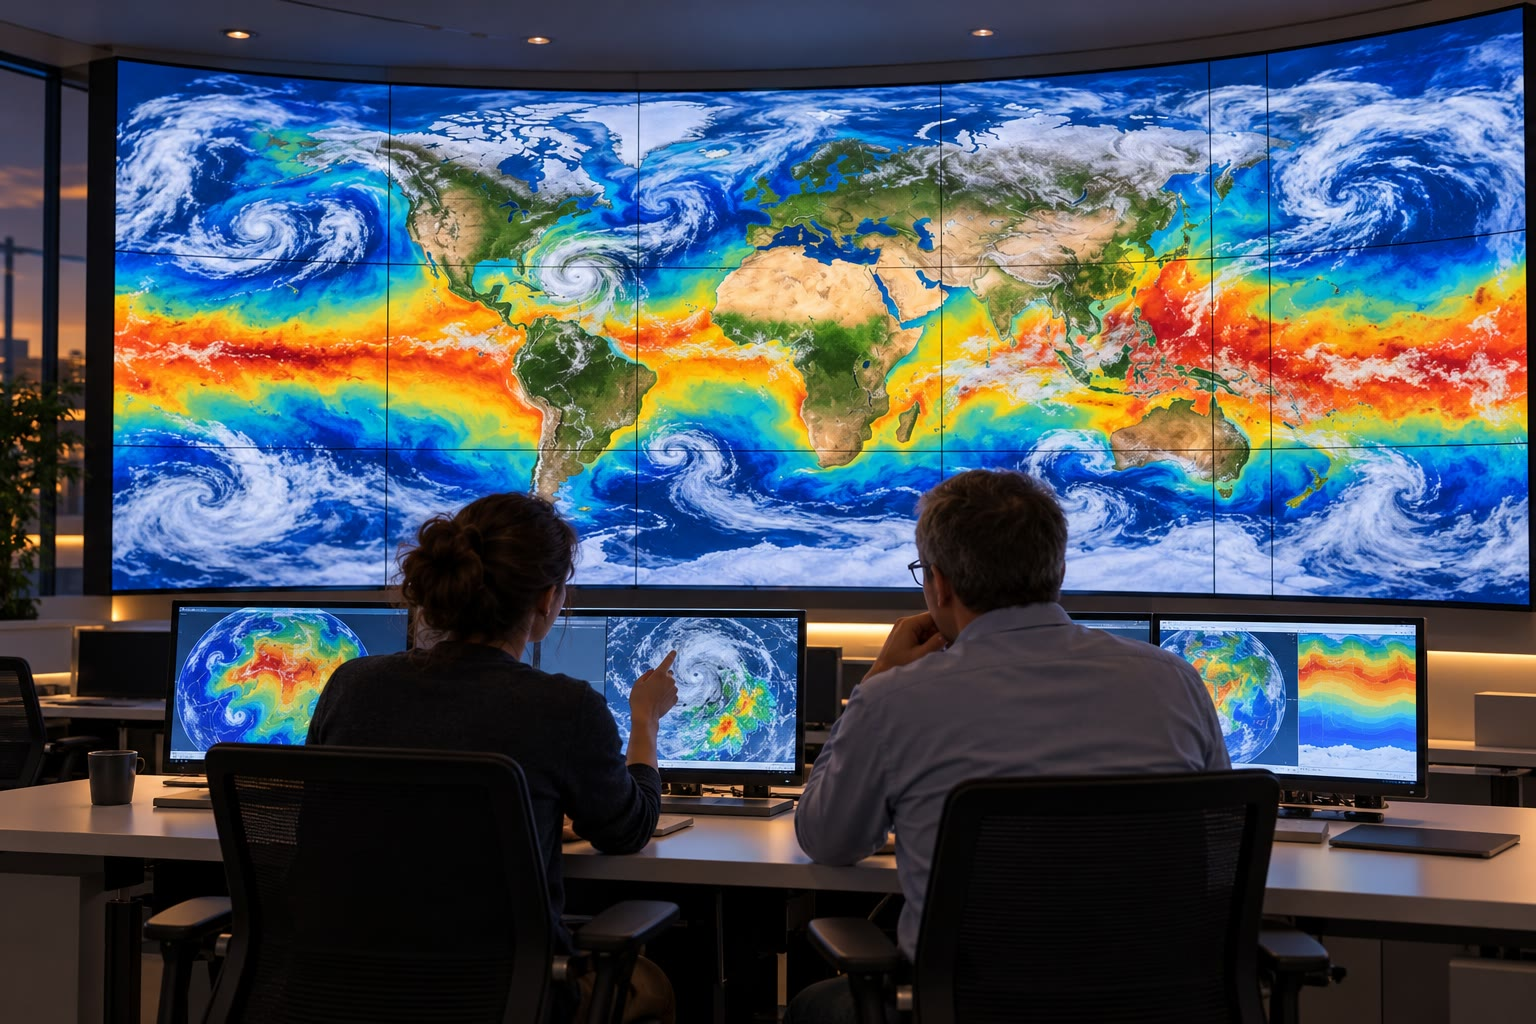
\includegraphics[width=\linewidth]{images/book5/ai/b3-model-centre.jpg}

{\scriptsize Two scientists in front of a wall of screens showing global
fields of a model run (AI-generated illustration).}
\end{minipage}
\end{inthelab}
% ledger: ar6ch1:esm, ar6ch1:models

\section{Exercises}

\begin{exercise}[$\star$]\label{exo:b3:climate-models:1}
Budyko's OLR law is $I = a + bT - (a_1 + b_1T)n$, with $a = 14.0$, $b =
0.14$, $a_1 = 3.0$, $b_1 = 0.10$, in \unit{kcal.cm^{-2}} per month and $T$
in \unit{\celsius}. For a cloudiness $n = 0.5$, compute $A$ and $B$, and
convert them to \unit{W/m^2} and \unit{W.m^{-2}.\celsius^{-1}}, with a
month a twelfth of a year of 365.25 days. What OLR does the law give at
\qty{15}{\celsius}?
\end{exercise}
% ledger: budyko69:olr

\begin{exercise}[$\star$]\label{exo:b3:climate-models:2}
With $Q = \qty{340}{W/m^2}$, $A = \qty{211.9}{W/m^2}$ and $B =
\qty{1.816}{W.m^{-2}.\celsius^{-1}}$, compute the equilibrium temperature
for an albedo of 0.30 and of 0.31. By how much does a rise of 0.01 of the
albedo cool this planet?
\end{exercise}

\begin{exercise}[$\star$]\label{exo:b3:climate-models:3}
Compute the heat capacity per square metre of a mixed layer of sea water
\qty{60}{m} deep, $\rho = \qty{1025}{kg/m^3}$ and $c_p = \qty{3992}{J.kg^{-1}.K^{-1}}$,
in \unit{J.m^{-2}.K^{-1}} and in \unit{W.yr.m^{-2}.K^{-1}}. Compute the
response time of \cref{thm:b3:climate-models:response} for $\lambda = -B =
\qty{-1.816}{W.m^{-2}.\celsius^{-1}}$ and for $\lambda =
\qty{-1.33}{W.m^{-2}.\celsius^{-1}}$.
\end{exercise}
% ledger: teos10:cp0

\begin{exercise}[$\star$]\label{exo:b3:climate-models:4}
For the two-layer model with $\lambda = \qty{-1.33}{W.m^{-2}.\celsius^{-1}}$,
$\gamma = \qty{0.62}{W.m^{-2}.\celsius^{-1}}$ and $F_{2\times} =
\qty{3.93}{W/m^2}$, compute the ECS, the approximate TCR $F_{2\times}/
(\gamma - \lambda)$, and their ratio.
\end{exercise}
% ledger: ar6sm7:two-layer, ipcc:erf-2xco2

\begin{exercise}[$\star\star$]\label{exo:b3:climate-models:5}
In the zero-dimensional model of the text, take a solar constant of
\qty{1340}{W/m^2}. Find the three equilibria and the slope $N'(T)$ of the
net flux at each; which are stable?
\end{exercise}

\begin{exercise}[$\star\star$]\label{exo:b3:climate-models:6}
Move the albedo ramp of the text: $\alpha = 0.62$ below \qty{-20}{\celsius},
$0.30$ above \qty{0}{\celsius}, linear between. Keep $A$ and $B$. At what
solar constant does the warm branch end, and by how many per cent is that
below \qty{1360}{W/m^2}? At what solar constant does the snowball melt?
What sets the size of the threshold?
\end{exercise}

\begin{exercise}[$\star\star$]\label{exo:b3:climate-models:7}
A model planet with the parameters of the text is in the snowball state.
(a)~What is its temperature at today's solar constant? (b)~Keeping the Sun
as it is, what forcing $F$ would bring the snowball's temperature up to
\qty{-10}{\celsius}? How many times the forcing of a doubling of carbon
dioxide, \qty{3.93}{W/m^2}, is it? (c)~Once the ice has gone, where does
the planet settle if the forcing is then removed?
\end{exercise}
% ledger: ipcc:erf-2xco2, hoffman17:hysteresis

\begin{exercise}[$\star\star$]\label{exo:b3:climate-models:8}
Model X, an invented two-layer model, has $C = 7.0$ and $C_d =
\qty{90}{W.yr.m^{-2}.\celsius^{-1}}$, $\gamma = 0.70$ and $\lambda =
\qty{-1.10}{W.m^{-2}.\celsius^{-1}}$. Compute its two time scales exactly
and with the approximations of \cref{thm:b3:climate-models:two-layer}, the
fraction $a_f$, its ECS and its approximate TCR.
\end{exercise}

\begin{exercise}[$\star\star$]\label{exo:b3:climate-models:9}
In Budyko's model of the text, $\bar T = \qty{12.81}{\celsius}$, $\beta =
\qty{3.74}{W.m^{-2}.\celsius^{-1}}$, the ice line at \ang{72}, $s = 1.221$
at the equator and $0.506$ at the pole, $\alpha = 0.30$ and $0.62$.
Compute the temperature at the equator and at the pole, and the heat
$\beta(T - \bar T)$ that the transport removes from, or brings to, each
square metre there.
\end{exercise}

\begin{exercise}[$\star\star\star$]\label{exo:b3:climate-models:10}
A planet without ice ($\alpha = 0.30$ everywhere) has the diffusive
transport $D = -\mathcal D\,\partial_x[(1 - x^2)\partial_xT]$ and the
insolation $s(x) = 1 + s_2P_2(x)$, $P_2 = (3x^2 - 1)/2$. (a)~Show that
$\partial_x[(1 - x^2)\partial_xP_2] = -6P_2$. (b)~Show that $T = T_0 +
T_2P_2(x)$ is a steady solution, with $T_0 = (Q(1 - \alpha) - A)/B$ and
$T_2 = Qs_2(1 - \alpha)/(B + 6\mathcal D)$. (c)~The insolation of the
reanalysis gives $s_2 = \num{-0.476}$. Without transport, what would be the
temperature difference between equator and pole? (d)~What $\mathcal D$ gives
the observed difference, \qty{55.3}{\celsius}?
\end{exercise}
% ledger: data:b3-ncep, data:b5-ncep-air

\begin{exercise}[$\star\star\star$]\label{exo:b3:climate-models:11}
(a)~Write the quadratic of \cref{thm:b3:climate-models:two-layer} as $r^2 -
\Sigma r + \Pi = 0$ and show that, if $4\Pi \ll \Sigma^2$, its roots are
close to $\Sigma$ and $\Pi/\Sigma$. (b)~For a forcing $F = kt$ rising
linearly, show that once $t \gg \tau_f$, and while $T_d$ stays small,
$T \approx kt/(\gamma - \lambda)$; deduce the approximate TCR. (c)~Check
the numbers of the text: $\Sigma$, $\Pi$, the two time scales, and the
ratio $4\Pi/\Sigma^2$.
\end{exercise}
% ledger: ar6sm7:two-layer

\begin{exercise}[$\star\star\star$]\label{exo:b3:climate-models:12}
An invented ensemble of eight models gives an observable $X$ of the
present climate and their ECS:
\begin{center}
\begin{tabular}{l*{8}{c}}
\hline
$X$ & 0.2 & 0.5 & 0.6 & 0.8 & 1.0 & 1.1 & 1.3 & 1.5\\
ECS (\unit{\celsius}) & 2.3 & 2.7 & 3.1 & 3.2 & 3.8 & 3.9 & 4.4 & 4.6\\
\hline
\end{tabular}
\end{center}
(a)~Compute the mean and the standard deviation of the ECS of the
ensemble. (b)~Fit ECS $= a + bX$ by least squares; compute the correlation
and the standard deviation of the residuals. (c)~The observed $X$ is $0.7
\pm 0.1$. What ECS does the constraint give, and with what spread?
(d)~What would make you distrust this constraint?
\end{exercise}
% ledger: ar6ch7:emergent

\section{Problem: How Close to a Snowball?}

\begin{problem}[{Weekend problem --- equilibria, stability and the
glaciation threshold of a model planet}]
\label{pb:b3:climate-models:1}
A model planet has today's solar constant $S_0 = \qty{1360}{W/m^2}$ and the
OLR law $A + BT$ with $A = \qty{211.9}{W/m^2}$ and $B =
\qty{1.816}{W.m^{-2}.\celsius^{-1}}$. Its albedo is 0.62 below
\qty{-10}{\celsius}, 0.30 above \qty{+10}{\celsius}, linear between, and
its surface heat capacity $C = \qty{8.1}{W.yr.m^{-2}.\celsius^{-1}}$. Take
$\sigma = \qty{5.670e-8}{W.m^{-2}.K^{-4}}$.

\medskip\noindent\textbf{Part I --- The planet in balance.}
\begin{enumerate}
\item Compute the mean sunlight $Q_0$ per square metre of the planet, and
  explain the factor.
\item Compute the absorbed sunlight with an albedo of 0.30, and the OLR at
  \qty{15}{\celsius}.
\item Compute the warm equilibrium.
\item Compute the snowball equilibrium, and check that it lies on the
  icy branch.
\item Compute the third equilibrium, on the albedo ramp.
\item Compute the emission temperature that sends the absorbed sunlight
  back to space as a black body, and compare it with the warm equilibrium.
\end{enumerate}

\medskip\noindent\textbf{Part II --- Stability and time.}
\begin{enumerate}[resume]
\item Compute the slope $N'(T)$ of the net flux at each equilibrium, and say
  which are stable.
\item A small departure from the middle equilibrium grows as $\mathrm
  e^{t/\tau}$. Compute $\tau$.
\item Compute the response time of the warm equilibrium.
\item A forcing of \qty{3.93}{W/m^2}, that of a doubling of carbon dioxide,
  is switched on. Compute the warming at equilibrium, and compare it with
  the ECS assessed for the real climate.
\item How long does the model take to cover \qty{95}{\percent} of the
  warming? Why does the real climate take longer?
\end{enumerate}

\medskip\noindent\textbf{Part III --- The saddle-node.}
\begin{enumerate}[resume]
\item As the Sun dims, at what temperature does the warm equilibrium meet
  the middle one? Compute $Q$ there.
\item Compute the solar constant at the bifurcation, and the drop from
  today in per cent.
\item Just below it, where does the climate go? Compute its temperature.
\item Compute the solar constant at which the snowball melts, and the rise
  from today in per cent.
\item Sketch the loop followed by the temperature when $S_0$ is lowered
  below the bifurcation and brought back to \qty{1360}{W/m^2}.
\end{enumerate}

\medskip\noindent\textbf{Part IV --- The ice line.} Give the planet
Budyko's latitudinal model, with $\beta = \qty{3.739}{W.m^{-2}.\celsius^{-1}}$,
an ice albedo of 0.62 poleward of the ice line, 0.30 equatorward, 0.50 at
the edge, and the insolation of the reanalysis:
\begin{center}
\begin{tabular}{lccccccc}
\hline
latitude & \ang{0} & \ang{30} & \ang{40} & \ang{47.5} & \ang{55} & \ang{60} & \ang{72}\\
$s(x_s)$ & 1.2211 & 1.0730 & 0.9647 & 0.8688 & 0.7650 & 0.6947 & 0.5643\\
$F(x_s)$ & 0 & 0.5865 & 0.7324 & 0.8192 & 0.8863 & 0.9205 & 0.9738\\
\hline
\end{tabular}
\end{center}
\begin{enumerate}[resume]
\item With the ice line at \ang{72}, compute the mean albedo $\bar\alpha$
  and the mean temperature $\bar T$.
\item Compute the critical temperature $T_c$ that puts the edge at
  \ang{72} today, and compare it with the reanalysis, \qty{-15.8}{\celsius}.
\item Compute the numerator of $Q(x_s)$ in \cref{prop:b3:climate-models:iceline}
  and the ratio $\beta/B$.
\item Compute $Q(x_s)/Q_0$ for the ice line at \ang{30}, \ang{40},
  \ang{47.5}, \ang{55} and \ang{60}.
\item Where is the minimum of these values? Which ice lines are stable?
\item With today's Sun, what other ice line does the model allow, and is
  it stable? Is the snowball possible today? (Use the column \ang{0}.)
\item Compare the threshold of the latitudinal model with that of Part~III
  and with Budyko's \qty{1.6}{\percent}, and the latitude of the ice at the
  threshold with his \ang{50}.
\item Give, to two significant figures, the fall of the solar constant, in
  per cent, that glaciates the model planet.
\end{enumerate}
\end{problem}
% ledger: nasa:solar-mean, data:b5-ncep-air, data:b3-ncep, budyko69:transport, budyko69:albedo, budyko69:threshold, ipcc:ecs, const:sigma
